% todos:
% - fisher z transformation einbauen
% effektstärkenkonvertierung: http://rwiki.sciviews.org/doku.php?id=packages:cran:ma_meta-analysis, http://cran.r-project.org/web/packages/metafor/metafor.pdf escalc

\documentclass[normalheadings, 10pt]{scrartcl}\usepackage{graphicx, color}
%% maxwidth is the original width if it is less than linewidth
%% otherwise use linewidth (to make sure the graphics do not exceed the margin)
\makeatletter
\def\maxwidth{ %
  \ifdim\Gin@nat@width>\linewidth
    \linewidth
  \else
    \Gin@nat@width
  \fi
}
\makeatother

\IfFileExists{upquote.sty}{\usepackage{upquote}}{}
\definecolor{fgcolor}{rgb}{0.2, 0.2, 0.2}
\newcommand{\hlnumber}[1]{\textcolor[rgb]{0,0,0}{#1}}%
\newcommand{\hlfunctioncall}[1]{\textcolor[rgb]{0.501960784313725,0,0.329411764705882}{\textbf{#1}}}%
\newcommand{\hlstring}[1]{\textcolor[rgb]{0.6,0.6,1}{#1}}%
\newcommand{\hlkeyword}[1]{\textcolor[rgb]{0,0,0}{\textbf{#1}}}%
\newcommand{\hlargument}[1]{\textcolor[rgb]{0.690196078431373,0.250980392156863,0.0196078431372549}{#1}}%
\newcommand{\hlcomment}[1]{\textcolor[rgb]{0.180392156862745,0.6,0.341176470588235}{#1}}%
\newcommand{\hlroxygencomment}[1]{\textcolor[rgb]{0.43921568627451,0.47843137254902,0.701960784313725}{#1}}%
\newcommand{\hlformalargs}[1]{\textcolor[rgb]{0.690196078431373,0.250980392156863,0.0196078431372549}{#1}}%
\newcommand{\hleqformalargs}[1]{\textcolor[rgb]{0.690196078431373,0.250980392156863,0.0196078431372549}{#1}}%
\newcommand{\hlassignement}[1]{\textcolor[rgb]{0,0,0}{\textbf{#1}}}%
\newcommand{\hlpackage}[1]{\textcolor[rgb]{0.588235294117647,0.709803921568627,0.145098039215686}{#1}}%
\newcommand{\hlslot}[1]{\textit{#1}}%
\newcommand{\hlsymbol}[1]{\textcolor[rgb]{0,0,0}{#1}}%
\newcommand{\hlprompt}[1]{\textcolor[rgb]{0.2,0.2,0.2}{#1}}%

\usepackage{framed}
\makeatletter
\newenvironment{kframe}{%
 \def\at@end@of@kframe{}%
 \ifinner\ifhmode%
  \def\at@end@of@kframe{\end{minipage}}%
  \begin{minipage}{\columnwidth}%
 \fi\fi%
 \def\FrameCommand##1{\hskip\@totalleftmargin \hskip-\fboxsep
 \colorbox{shadecolor}{##1}\hskip-\fboxsep
     % There is no \\@totalrightmargin, so:
     \hskip-\linewidth \hskip-\@totalleftmargin \hskip\columnwidth}%
 \MakeFramed {\advance\hsize-\width
   \@totalleftmargin\z@ \linewidth\hsize
   \@setminipage}}%
 {\par\unskip\endMakeFramed%
 \at@end@of@kframe}
\makeatother

\definecolor{shadecolor}{rgb}{.97, .97, .97}
\definecolor{messagecolor}{rgb}{0, 0, 0}
\definecolor{warningcolor}{rgb}{1, 0, 1}
\definecolor{errorcolor}{rgb}{1, 0, 0}
\newenvironment{knitrout}{}{} % an empty environment to be redefined in TeX

\usepackage{alltt}

\usepackage[T1]{fontenc}
\usepackage[utf8x]{inputenc}

\usepackage[ngerman]{babel}

\usepackage{csquotes}

\usepackage{helvet}

\usepackage{graphicx}
\graphicspath{{fig/}}



\newcommand{\code}[1]{\texttt{#1}}

\title{Übungen zum GESIS Workshop \enquote{Grundlagen sozialwissenschaftlicher Meta-Analysen}}
\author{Bernd Weiß}

\usepackage{listings}
\lstset{%
  basicstyle=\ttfamily
}

\usepackage{geometry}
\geometry{a4paper,left=35mm,right=20mm, top=15mm, bottom=20mm}


\usepackage{tcolorbox}
\tcbset{before={\par\medskip\pagebreak[0]\noindent},after={\par\medskip}}%
% \newenvironment{rbsp}{%
%   \tcolorbox[savedelimiter=mybox,
%   lowerbox=ignored,
%   colback=white,colframe=gray!75!black,fonttitle=\bfseries\textsf,title=R Beispiel]}%
% {\endtcolorbox}

% \usepackage{color}
% \newenvironment{rbsp}{%
%   \vspace{2ex} \hspace{-0.51cm}
%   \vspace{-0.41cm} \noindent  \colorbox{gray}{\color{white}{\textsf{R Beispiel}}}
%   \begin{oframed}}{\end{oframed}}

\usepackage{mdframed}

\newmdenv[outerlinewidth=0,
          %% nobreak = true,
          font=\footnotesize,
          leftmargin=40,%
          rightmargin=0,
          backgroundcolor=white,%
          outerlinecolor=black,
          innertopmargin=-2ex,%
          innerbottommargin=-3ex,%
          splittopskip=1ex,
          skipbelow=3ex,%
          skipabove=3ex,
          %frametitleaboveskip=-0.3cm,
          frametitlerule=true,
          linewidth=0.5pt,
          frametitle={\textsf{R Beispiel}}]{rbsp}


\newmdenv[outerlinewidth=0,
          font=\footnotesize,
          leftmargin=40,%
          rightmargin=0,
          backgroundcolor=white,%
          outerlinecolor=black,
          innertopmargin=1ex,%
          innerbottommargin=1ex,%
          splittopskip=1ex,
          skipbelow=3ex,%
          skipabove=3ex,
          %frametitleaboveskip=-0.3cm,
          frametitlerule=true,
          linewidth=0.5pt,
          frametitle={\textsf{Stata Beispiel}}]{statabsp}


% \newenvironment{statabsp}{%
%   \tcolorbox[savedelimiter=mybox,
%   lowerbox=ignored,
%   colback=white,colframe=gray!75!black,fonttitle=\bfseries\textsf,title=Stata Beispiel]}%
% {\endtcolorbox}









\hyphenation{z-Trans-for-ma-tion}

\begin{document}


\maketitle

\tableofcontents

\vspace{10ex}

\section*{Vorbemerkungen}

In den praktischen Übungen wird der Schwerpunkt auf dem Umgang mit der Software
R liegen. In einigen (komplexeren) oder ausdrücklich meta-analytischen Fällen wird sowohl der R- als auch der
Stata-Code vorgestellt.

In den "`R Code-Boxen"' wird sowohl die R-Eingabe als auch die -Ausgabe
("`Output"') dargestellt. Sämtliche Ausgaben (meistens die Ergebnisse von
Berechnungen) beginnen mit dem sogenannten "`R prompt"': \texttt{R> }. Manchmal
wird nach dem Prompt noch eine Zahl in eckigen Klammern dargestellt, etwa
\texttt{R> [1]}. Für Vektoren (also mehrere Zahlen) geben die Zahlen in den
eckigen Klammern an, das wievielte Element am Anfang der jeweiligen Zeile zu
finden ist (siehe bspw. Aufgabe 1-1-3).

Es werden zahlreiche neue R-/Stata-Befehle eingeführt. In der
Aufgabenbeschreibung wird ein neuer Befehl mindestens einmal aufgeführt, aber
zumeist nicht weiter erläutert. Zusätzliche Hinweise zur Verwendung der Befehle
finden sich dann im Programmcode in den Kommentaren.

%Code extraction assignmentsession..chunk, assing-2.1.a
% tag-teil-laufendenummer



\section{Übung 1-1}

\subsection{Der erste Kontakt mit R}


\paragraph{Aufgabe 1-1-1} Berechnen Sie die Summe aus 123 + 789 und weisen Sie das Ergebnis einer
  Variablen \code{x} zu. Tippen Sie anschließend \code{x} ein und lassen Sie
  sich das Ergebnis Ihrer Berechnung anzeigen.

\begin{rbsp}
\begin{knitrout}
\definecolor{shadecolor}{rgb}{1, 1, 1}\color{fgcolor}\begin{kframe}
\begin{verbatim}
x <- 123 + 789
x
R>  [1] 912
\end{verbatim}
\end{kframe}
\end{knitrout}

\end{rbsp}


\paragraph{Aufgabe 1-1-2} Bestimmen Sie das Quadrat von \code{x}, also
\verb|x^2| (das Zeichen \code{\^} finden sie links oben, unterhalb der
ESC-Taste).

\begin{rbsp}
\begin{knitrout}
\definecolor{shadecolor}{rgb}{1, 1, 1}\color{fgcolor}\begin{kframe}
\begin{verbatim}
x^2
R>  [1] 831744
\end{verbatim}
\end{kframe}
\end{knitrout}

\end{rbsp}


\paragraph{Aufgabe 1-1-3} Erzeugen Sie mit dem Ausdruck \code{1:10} die
Zahlensequenz von 1 bis 10 und weisen Sie diese der Variablen \code{myseq}
zu. Berechnen Sie anschließend die quadrierte Inverse (für $a$ ist das
$1/a^2$) für jedes Element des Vektors.

\begin{rbsp}
\begin{knitrout}
\definecolor{shadecolor}{rgb}{1, 1, 1}\color{fgcolor}\begin{kframe}
\begin{verbatim}
myseq <- 1:10
1/(myseq^2)
R>   [1] 1.00000 0.25000 0.11111 0.06250 0.04000 0.02778 0.02041 0.01562
R>   [9] 0.01235 0.01000
\end{verbatim}
\end{kframe}
\end{knitrout}

\end{rbsp}


\subsection{Effektstärken}

\paragraph{Aufgabe 1-1-4} In einer Studie werden zwei Gruppen bezüglich ihres Mittelwertes
  verglichen. Sie finden Angaben zu den beiden Mittelwerten, $Y_1 = 103$ und
  $Y_2=100$, den beiden Standardabweichungen, $S_1=5.5$ und $S_2=4.5$, sowie den
  Fallzahlen, $n_1=n_2=50$. Ermitteln Sie die unstandardisierte
  Mittelwertdifferenz sowie deren Standardfehler. Weiterhin wird angenommen,
  dass sich die beiden Populationsvarianzen nicht unterscheiden, also $\sigma_1=\sigma_2$

\begin{rbsp}
\begin{knitrout}
\definecolor{shadecolor}{rgb}{1, 1, 1}\color{fgcolor}\begin{kframe}
\begin{verbatim}
y1 <- 103
y2 <- 100
s1 <- 5.5
s2 <- 4.5
n1 <- n2 <- 50 ## "Doppelzuweisung"

## Berechne die Mittelwertdifferenz (Eine Klammer (...)
## um diesen Ausdruck bedeutet "print()")
(D <- y1 - y2)
R>  [1] 3

s.pooled <- sqrt(((n1-1)*s1^2 + (n2-1)*s2^2)/(n1+n2-2))

vd <- s.pooled^2 * (n1+n2)/(n1*n2)

## Mittelwertdifferenz:
D
R>  [1] 3

## Varianz:
vd
R>  [1] 1.01
\end{verbatim}
\end{kframe}
\end{knitrout}

\end{rbsp}


\paragraph{Aufgabe 1-1-5} Sie erinnern sich (hoffentlich) noch daran, dass Korrelationen im Rahmen
  einer Meta-Analyse häufig erst transformiert werden müssen (Fisher's
  z-Trans\-for\-ma\-tion). Gegeben sind $r=0.50$ und $N=100$. Berechnen Sie z sowie
  den dazugehörigen Standardfehler.

\begin{rbsp}
\begin{knitrout}
\definecolor{shadecolor}{rgb}{1, 1, 1}\color{fgcolor}\begin{kframe}
\begin{verbatim}
r <- 0.50
N <- 100

r.z <- 0.5*log((1+r)/(1-r))
r.z
R>  [1] 0.5493

var.r.z <- 1/(N-3)
var.r.z
R>  [1] 0.01031
sqrt(var.r.z)
R>  [1] 0.1015
\end{verbatim}
\end{kframe}
\end{knitrout}

\end{rbsp}

%% Paket muss 2x geladen werden, um den §"%&§$ output zu uenterdrucken...



Zum Glück muss das Rad nicht neu erfunden werden und es gibt in R bereits
Funktionen, die die Fisher's z-Transformation durchführen. Dazu muss allerdings
zunächst das Paket \texttt{psychometric} geladen werden.

\begin{rbsp}
\begin{knitrout}
\definecolor{shadecolor}{rgb}{1, 1, 1}\color{fgcolor}\begin{kframe}
\begin{verbatim}

library(psychometric)

(r.z <- r2z(r))
R>  [1] 0.5493
SEz(N)
R>  [1] 0.1015
z2r(r.z)
R>  [1] 0.5
\end{verbatim}
\end{kframe}
\end{knitrout}

\end{rbsp}


\paragraph{Aufgabe 1-1-6} Normalerweise kommt in einer Meta-Analysen nicht nur
\emph{ein} Korrelationskoeffizient vor, sondern es gibt mehrere davon (in R spricht man
von einem Vektor = Variable). Die bislang vorgestellten
Vorgehensweisen/Funktionen funktionieren natürlich auch für Vektoren.

\begin{rbsp}
\begin{knitrout}
\definecolor{shadecolor}{rgb}{1, 1, 1}\color{fgcolor}\begin{kframe}
\begin{verbatim}
r <- c(0.5, 0.4, 0.1)
N <- c(100, 102, 110)

r2z(r)
R>  [1] 0.5493 0.4236 0.1003
SEz(N)
R>  [1] 0.10153 0.10050 0.09667
\end{verbatim}
\end{kframe}
\end{knitrout}

\end{rbsp}


Auch in Stata lässt sich die Fisher's z-Transformation durchführen:


\begin{statabsp}
  \lstinputlisting{../stata/assign-1-1-6.do}
\end{statabsp}



\paragraph{Aufgabe 1-1-7} Zum Abschluss soll ein kurzer Ausblick auf
Effektstärkenkonvertierungen gegeben werden. Zunächst wird ein etwas
aufwändigeres Vorgehen beschrieben, das aber ohne die Verwendung eines
Zusatzpaketes auskommt.\footnote{Es gibt in R auch noch das Paket
  \texttt{compute.es}, das solche Transformationen ermöglicht.}

Gegeben ist ein $ln(Odds Ratio)$ von $0.9069$, mit einer Varianz von $0.0676$, und
diese Angaben sollen nach Cohens $d$ konvertiert werden.

\begin{rbsp}
\begin{knitrout}
\definecolor{shadecolor}{rgb}{1, 1, 1}\color{fgcolor}\begin{kframe}
\begin{verbatim}
lnor <- 0.9069
V.lnor <- 0.0676

d <- lnor * (sqrt(3)/pi)
d
R>  [1] 0.5

V.d <- V.lnor * (3/pi^2)
V.d
R>  [1] 0.02055
\end{verbatim}
\end{kframe}
\end{knitrout}

\end{rbsp}


An diesem Beispiel soll auch die Verwendung von eigenen Funktionen in R illustriert
werden. Das heißt, es wird eine eigene "`ln(Odds Ratio) nach d"'-Funktion
erstellt:

\begin{rbsp}
\begin{knitrout}
\definecolor{shadecolor}{rgb}{1, 1, 1}\color{fgcolor}\begin{kframe}
\begin{verbatim}

lor2d <- function(lor, V){
    d <- lor * (sqrt(3)/pi)
    V.d <- V * (3/pi^2)
    res <- c(d=d, Var=V.d)
    return(res)
}

coh.d <- lor2d(lnor, V.lnor)
coh.d
R>        d     Var 
R>  0.50000 0.02055

coh.d[1]
R>    d 
R>  0.5
coh.d[2]
R>      Var 
R>  0.02055
\end{verbatim}
\end{kframe}
\end{knitrout}

\end{rbsp}


\subsection{Effektstärkenverteilungen I}

Im Folgenden soll eine univariate Meta-Analyse mit den
Daten von Aloe/Becker (2009, "`Teacher Verbal Ability and School Outcomes"')
durchgeführt werden.


\paragraph{Aufgabe 1-1-9} Laden Sie den Datensatz
\texttt{uebung1-1-9\_dVerbAb.csv} (PM-Korrelationen zwischen "`teacher verbal
ability"' und verschiedenen "`school autcomes"'; dieser Datensatz ist im
Verzeichnis \texttt{data/} zu finden). Verwenden Sie dazu die Funktion
\code{read.csv(\ldots)}. Die Daten liegen im csv-Format (csv = comma-separated
values) vor. Mit dem Argument \code{file = "\ldots"} geben Sie an, wo R die
Daten finden kann (auf den GESIS-Computern ist das sicher nicht
\code{"../../data/"}, siehe Beispiel).

In unserem Fall ist der Spaltentrenner das Semikolon (;). Denken Sie daran, dass
Sie beim Laden des Datensatzes diesen einem R-Objekt zuweisen müssen (verwenden
Sie z.B. den Namen \code{dfVerb}). Lassen Sie sich anschließend den Inhalt des
Objektes \code{dfVerb} anzeigen.

\begin{rbsp}
\begin{knitrout}
\definecolor{shadecolor}{rgb}{1, 1, 1}\color{fgcolor}\begin{kframe}
\begin{verbatim}
dfVerb <- read.csv(file = "../../data/uebung1-1-9_dVerbAb.csv", sep = ";")
dfVerb
R>     ID year     r   N
R>  1   1 1980 -0.10   7
R>  2   2 2005  0.23  76
R>  3   4 1968 -0.05 155
R>  4   5 1968  0.02  45
R>  5   6 1969 -0.09  31
R>  6   7 1969  0.26  37
R>  7   9 1970 -0.07  79
R>  8  10 1987  0.04 151
R>  9  11 1987 -0.01 151
R>  10 12 1993  0.12  64
R>  11 13 1991  0.03 318
R>  12 14 1988  0.07 288
R>  13 15 1988 -0.05  31
R>  14 16 1966  0.13 500
R>  15 17 1966  0.03 500
R>  16 18 1966  0.21 500
R>  17 19 1966  0.28 500
\end{verbatim}
\end{kframe}
\end{knitrout}

\end{rbsp}

\pagebreak

\paragraph{Aufgabe 1-1-10} Als nächstes müssen die Korrelationen
Fisher-z-transformiert werden. Dazu verwenden wir die Funktion \code{r2z}, die
im Paket \code{psychometric} zu finden ist. Um den Standardfehler für die neue
Effektstärke $z_r$ zu berechnen, kann die Funktion \code{SEz} benutzt
werden. Der Standardfehler ist in diesem Fall nur eine Funktion der Fallzahl,
also benötigen wir nur die Variable \code{N}.

\begin{rbsp}
\begin{knitrout}
\definecolor{shadecolor}{rgb}{1, 1, 1}\color{fgcolor}\begin{kframe}
\begin{verbatim}
library(psychometric)

## Geben Sie einfach nur den Namen der Funktion r2z ein. Kommt Ihnen
## das bekannt vor?
r2z
R>  function (x) 
R>  {
R>      0.5 * log((1 + x)/(1 - x))
R>  }
R>  <environment: namespace:psychometric>

## Nun die Fisher-z-Trasformation durchfuehren. Die neue Variable soll
## im Datensatz dfVerb gespeichert werden.
dfVerb$z.r <- r2z(dfVerb$r)

## Den Standardfehler von r.z ermitteln:
dfVerb$se.z <- SEz(dfVerb$N)

## Den erweiterten Datensatz anzeigen lassen:
dfVerb
R>     ID year     r   N      z.r    se.z
R>  1   1 1980 -0.10   7 -0.10034 0.50000
R>  2   2 2005  0.23  76  0.23419 0.11704
R>  3   4 1968 -0.05 155 -0.05004 0.08111
R>  4   5 1968  0.02  45  0.02000 0.15430
R>  5   6 1969 -0.09  31 -0.09024 0.18898
R>  6   7 1969  0.26  37  0.26611 0.17150
R>  7   9 1970 -0.07  79 -0.07011 0.11471
R>  8  10 1987  0.04 151  0.04002 0.08220
R>  9  11 1987 -0.01 151 -0.01000 0.08220
R>  10 12 1993  0.12  64  0.12058 0.12804
R>  11 13 1991  0.03 318  0.03001 0.05634
R>  12 14 1988  0.07 288  0.07011 0.05923
R>  13 15 1988 -0.05  31 -0.05004 0.18898
R>  14 16 1966  0.13 500  0.13074 0.04486
R>  15 17 1966  0.03 500  0.03001 0.04486
R>  16 18 1966  0.21 500  0.21317 0.04486
R>  17 19 1966  0.28 500  0.28768 0.04486
\end{verbatim}
\end{kframe}
\end{knitrout}

\end{rbsp}

\pagebreak

\paragraph{Aufgabe 1-1-11} Vor der eigentlichen Meta-Analyse untersuchen wir
etwas genauer den Zusammenhang zwischen $r$ und $z_r$, erstellen ein Histogramm
der $z_r$ und lernen damit einfache Grafikbefehle in R. Was fällt Ihnen auf?

\begin{rbsp}
\begin{knitrout}
\definecolor{shadecolor}{rgb}{1, 1, 1}\color{fgcolor}\begin{kframe}
\begin{verbatim}
plot(x = dfVerb$r, y = dfVerb$z.r, xlab = "r", ylab = "Fisher's z",
     main = "Zusammenhang zwischen r und z.r")
\end{verbatim}
\end{kframe}
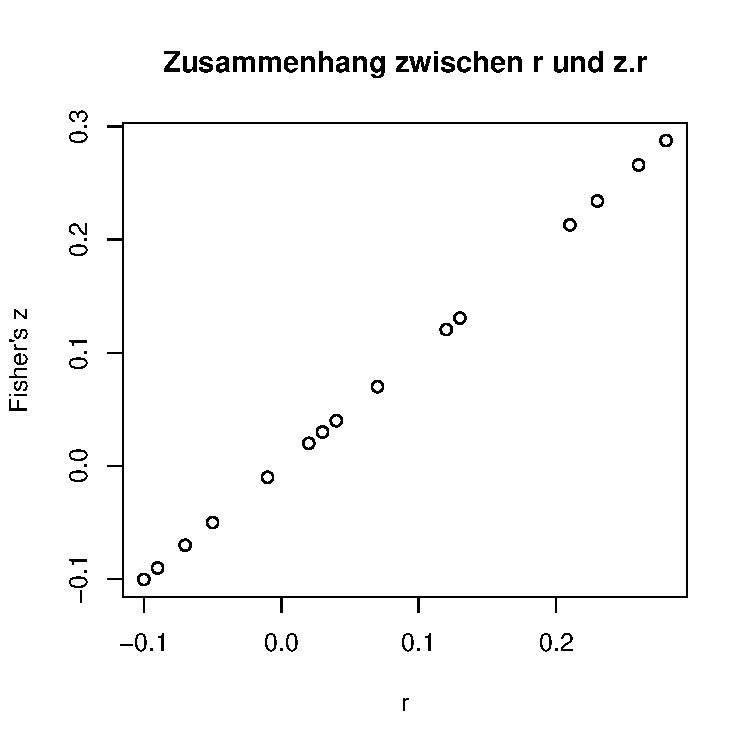
\includegraphics[width=\maxwidth]{fig/assign-1-1-11_1} 

\end{knitrout}

\end{rbsp}

\pagebreak

Als nächstes schauen wir uns die Verteilung der Effektstärken genauer
an. Histogramme lassen sich in R mit dem Befehl \code{hist(\ldots)} erstellen.

\begin{rbsp}
\begin{knitrout}
\definecolor{shadecolor}{rgb}{1, 1, 1}\color{fgcolor}\begin{kframe}
\begin{verbatim}
hist(dfVerb$z.r)
\end{verbatim}
\end{kframe}
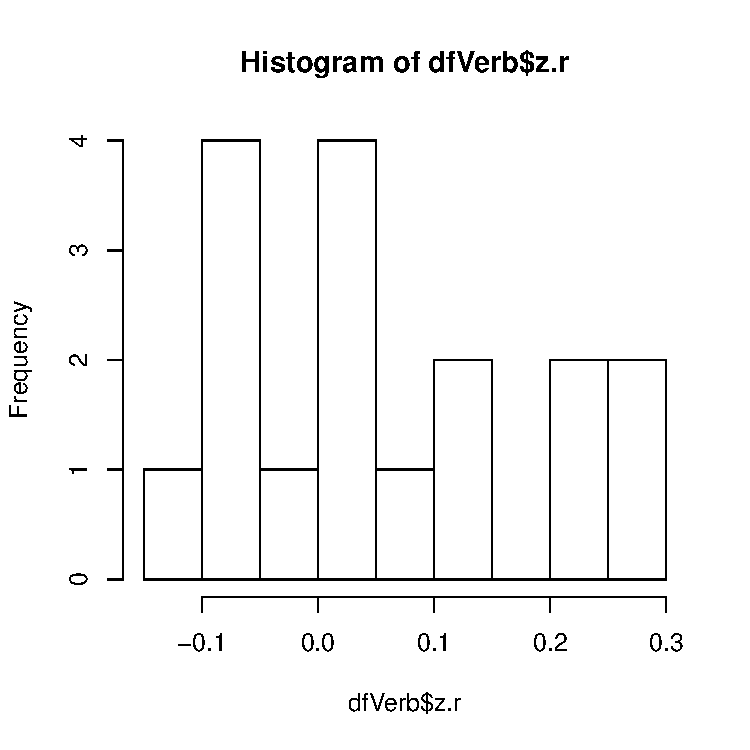
\includegraphics[width=\maxwidth]{fig/assign-1-1-11_2} 

\end{knitrout}

\end{rbsp}

\pagebreak

Ist die Variable normalverteilt? Es wird vermutlich auch nicht besser, wenn wir
das Histogramm um einen Dichteplot erweitern:

\begin{rbsp}
\begin{knitrout}
\definecolor{shadecolor}{rgb}{1, 1, 1}\color{fgcolor}\begin{kframe}
\begin{verbatim}
## Mit dem Argument freq = FALSE wird im Histogramm nicht die absolute
## Haeufigkeit sondern die Wahrscheinlichkeitsdichte dargestellt
## Mit xlim = ... geben wir die Begrenzungen der x-Achse an.
hist(dfVerb$z.r, freq = FALSE, xlim = c(-0.3, 0.4), xlab = "Fisher's z",
     ylab = "Dichte", main = "")

## Zunächst wird die Wahrschenlichkeitsdichte geschaetzt
tmp <- density(dfVerb$z.r)

## Mit der lines()-Funktion wird zu einem bestehenden Plot ein Linien-
## plot hinzugefuegt
lines(tmp)
\end{verbatim}
\end{kframe}
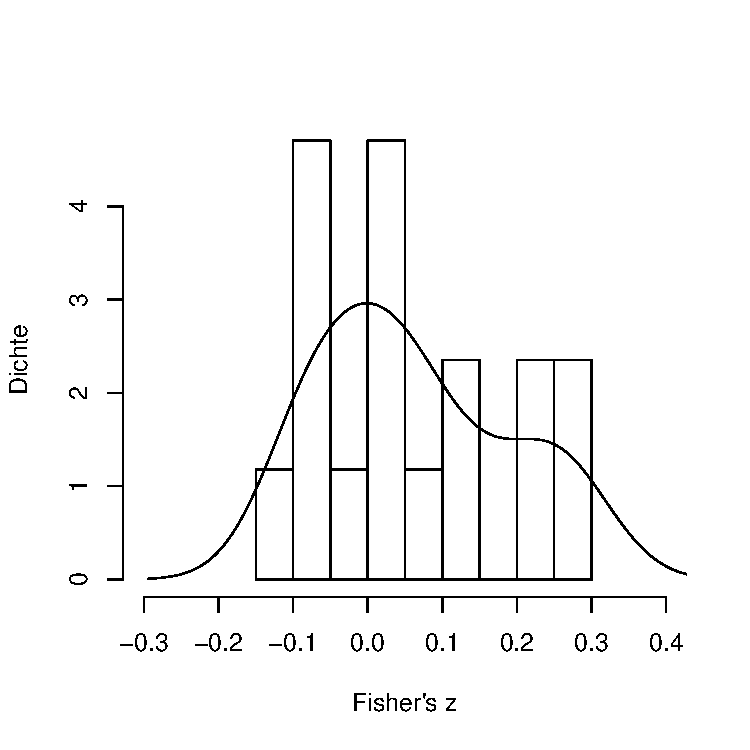
\includegraphics[width=\maxwidth]{fig/assign-1-1-11_3} 

\end{knitrout}

\end{rbsp}

\pagebreak

\section{Übung 2-1}

\subsection{Effektstärkenverteilungen II}



\paragraph{Aufgabe 2-1-1} Kommen wir nun zur eigentlichen Meta-Analyse. Wie Sie
den Folien (Kapitel 17: Meta-Analyse-Software für R und Stata) entnehmen können
gibt es für R mehrere Pakete, mit denen sich univariate Meta-Analysen
durchführen lassen. Das von mir bevorzugte Paket heißt \code{meta} und die
Funktion zur Durchführung einer Meta-Analyse heißt \code{metagen} (gen =
generisch) .

\begin{rbsp}
\begin{knitrout}
\definecolor{shadecolor}{rgb}{1, 1, 1}\color{fgcolor}\begin{kframe}
\begin{verbatim}
library(meta)
\end{verbatim}


{\ttfamily\noindent\itshape\textcolor{messagecolor}{R>  Loading required package: grid}}

{\ttfamily\noindent\itshape\textcolor{messagecolor}{R>  Loading 'meta' package (version 2.1-4).}}\begin{verbatim}

## Ein
metagen(TE = z.r, seTE = se.z, data = dfVerb)
R>                         95%-CI %W(fixed) %W(random)
R>  1  -0.1003  [-1.0803; 0.8796]      0.12       0.38
R>  2   0.2342  [ 0.0048; 0.4636]      2.16       4.52
R>  3  -0.0500  [-0.2090; 0.1089]      4.49       6.72
R>  4   0.0200  [-0.2824; 0.3224]      1.24       3.09
R>  5  -0.0902  [-0.4606; 0.2802]      0.83       2.25
R>  6   0.2661  [-0.0700; 0.6022]      1.01       2.63
R>  7  -0.0701  [-0.2949; 0.1547]      2.25       4.64
R>  8   0.0400  [-0.1211; 0.2011]      4.38       6.63
R>  9  -0.0100  [-0.1711; 0.1511]      4.38       6.63
R>  10  0.1206  [-0.1304; 0.3715]      1.80       4.02
R>  11  0.0300  [-0.0804; 0.1404]      9.31       8.74
R>  12  0.0701  [-0.0460; 0.1862]      8.43       8.49
R>  13 -0.0500  [-0.4204; 0.3204]      0.83       2.25
R>  14  0.1307  [ 0.0428; 0.2187]     14.70       9.75
R>  15  0.0300  [-0.0579; 0.1179]     14.70       9.75
R>  16  0.2132  [ 0.1253; 0.3011]     14.70       9.75
R>  17  0.2877  [ 0.1998; 0.3756]     14.70       9.75
R>  
R>  Number of studies combined: k=17
R>  
R>                                         95%-CI     z  p.value
R>  Fixed effect model   0.1123  [0.0786; 0.1460] 6.530 < 0.0001
R>  Random effects model 0.0880  [0.0265; 0.1495] 2.803   0.0051
R>  
R>  Quantifying heterogeneity:
R>  tau^2 = 0.0081; H = 1.59 [1.22; 2.07]; I^2 = 60.4% [32.6%; 76.7%]
R>  
R>  Test of heterogeneity:
R>       Q d.f.  p.value
R>   40.36   16   0.0007
R>  
R>  Details on meta-analytical method:
R>  - Inverse variance method
R>  - DerSimonian-Laird estimator for tau^2
\end{verbatim}
\end{kframe}
\end{knitrout}

\end{rbsp}

\code{metagen()} produziert eine Menge Zahlen, daher sollen Ihnen die
folgenden Fragen helfen, die Ausgabe zu interpretieren:

\begin{itemize}
\item Welches Effektstärkenmodell ist \emph{empirisch} angemessen? Welche
  Heterogenitätsstatistiken geben darüber Auskunft?
\item Ist die zusammengefasste Effektstärke statistisch signifikant?
\item Welche Informationen liefern die beiden mit \code{\%W(fixed)} und
  \code{\%W(random)} überschriebenen Spalten der Tabelle? Wenn Sie die beiden
  Spalten vergleichen, was fällt Ihnen auf? Haben Sie eine Erklärung dafür?
\end{itemize}

Angenommen, Sie haben sich für den REM-Schätzer entschieden und möchten ihn nun
in einer Publikation darstellen. Verwenden Sie dafür den transformierten Wert
oder ist es nicht angemessener, den Gesamteffekt in die originale
Korrelationsskala zurückzutransformieren? Korrekt, Sie möchten einen
Korrelationskoeffizienten darstellen. Dazu müssen wir den REM Schätzer mit der
Funktion \code{z2r} des Paketes \code{psychometric} zurücktransformieren.


\begin{rbsp}
\begin{knitrout}
\definecolor{shadecolor}{rgb}{1, 1, 1}\color{fgcolor}\begin{kframe}
\begin{verbatim}
## Sie koennen den REM Schaetzer natuerlich auch von Hand eintippen, aber
## besser ist es, das Ergebnis der Meta-Analyse in einem Objekt tmp zu
## speichern und dieses Objekt enthaelt auch die entsprechenden Angaben
tmp <- metagen(TE = z.r, seTE = se.z, data = dfVerb)

## Mit der Funktion str() koennen Sie sich anzeigen lassen, was in tmp
## enthalten ist. Aus Platzgruenden wird der folgende Befehl nicht ausgefuehrt:
## str(tmp)

## Sieht zunaechst verwirrend aus, aber schlussendlich findet sich in der
## Zeile " TE.random : num 0.088" das, was wir suchen, naemlich der Name
## des Listenelementes "TE.random".
tmp$TE.random
R>  [1] 0.08798

## Schliesslich die Ruecktransformation:
z2r(tmp$TE.random)
R>  [1] 0.08775
\end{verbatim}
\end{kframe}
\end{knitrout}

\end{rbsp}

Nach diesem (didaktisch wertvollen) Aufwand mit Fisher-z-Transformation,
Standardfehlerberchnung und Rücktransformation möchte ich Ihnen abschließend die
Funktion \code{metacor} vorstellen, die das alles in einer Zeile erledigt:

\begin{rbsp}
\begin{knitrout}
\definecolor{shadecolor}{rgb}{1, 1, 1}\color{fgcolor}\begin{kframe}
\begin{verbatim}
metacor(cor = r, n = N, data = dfVerb)
R>       COR             95%-CI %W(fixed) %W(random)
R>  1  -0.10  [-0.7933; 0.7062]      0.12       0.38
R>  2   0.23  [ 0.0048; 0.4330]      2.16       4.52
R>  3  -0.05  [-0.2060; 0.1085]      4.49       6.72
R>  4   0.02  [-0.2751; 0.3117]      1.24       3.09
R>  5  -0.09  [-0.4306; 0.2730]      0.83       2.25
R>  6   0.26  [-0.0699; 0.5386]      1.01       2.63
R>  7  -0.07  [-0.2867; 0.1535]      2.25       4.64
R>  8   0.04  [-0.1205; 0.1985]      4.38       6.63
R>  9  -0.01  [-0.1695; 0.1500]      4.38       6.63
R>  10  0.12  [-0.1296; 0.3553]      1.80       4.02
R>  11  0.03  [-0.0802; 0.1395]      9.31       8.74
R>  12  0.07  [-0.0460; 0.1841]      8.43       8.49
R>  13 -0.05  [-0.3973; 0.3098]      0.83       2.25
R>  14  0.13  [ 0.0428; 0.2152]     14.70       9.75
R>  15  0.03  [-0.0578; 0.1174]     14.70       9.75
R>  16  0.21  [ 0.1246; 0.2923]     14.70       9.75
R>  17  0.28  [ 0.1972; 0.3589]     14.70       9.75
R>  
R>  Number of studies combined: k=17
R>  
R>                          COR            95%-CI     z  p.value
R>  Fixed effect model   0.1118  [0.0784; 0.1450] 6.530 < 0.0001
R>  Random effects model 0.0878  [0.0265; 0.1484] 2.803   0.0051
R>  
R>  Quantifying heterogeneity:
R>  tau^2 = 0.0081; H = 1.59 [1.22; 2.07]; I^2 = 60.4% [32.6%; 76.7%]
R>  
R>  Test of heterogeneity:
R>       Q d.f.  p.value
R>   40.36   16   0.0007
R>  
R>  Details on meta-analytical method:
R>  - Inverse variance method
R>  - DerSimonian-Laird estimator for tau^2
R>  - Fisher's z transformation of correlations
\end{verbatim}
\end{kframe}
\end{knitrout}

\end{rbsp}

Bevor ich die entsprechenden Schritte in Stata vorstelle, möchte ich noch zeigen,
wie in R ein Forestplot erstellt wird. Dazu verwende ich den Befehl
\code{forest()}. Die meisten Argumente dieser Funktion sprechen für sich
selbst. Mit \code{hetstat = FALSE} wird verhindert, dass verschiedene
zusätzliche Heterogenitätsstatistiken aufgeführt werden. Wenn Sie sich mit
\code{?forest} die Hilfeseiten dieser Funktion anschauen, dann werden Sie
feststellen, dass dieser Befehl sehr umfangreich ist.


\begin{rbsp}
\begin{knitrout}
\definecolor{shadecolor}{rgb}{1, 1, 1}\color{fgcolor}\begin{kframe}
\begin{verbatim}
tmp <- metacor(cor = r, n = N, data = dfVerb)
forest(tmp, main = "", smlab = "Fisher's z", leftcols = c("studlab"),
       text.fixed = "FEM", text.random = "REM", pooled.total = FALSE,
       hetstat = FALSE )
\end{verbatim}
\end{kframe}
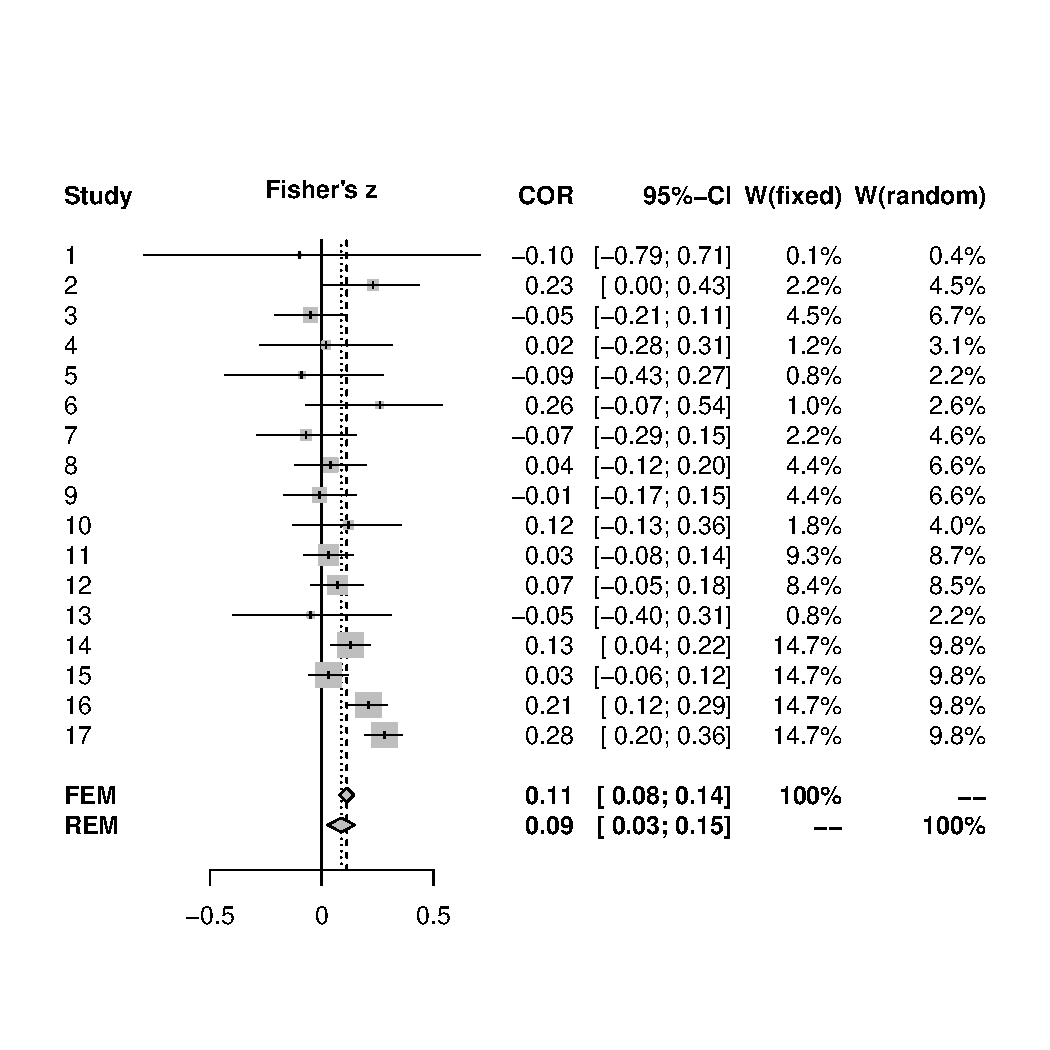
\includegraphics[width=\maxwidth]{fig/assign-2-1-1_4} 

\end{knitrout}

\end{rbsp}


Abschließend noch das entsprechende Vorgehen in Stata. Sie müssen dazu das Stata
add-on \code{metan} installiert haben (Installation erfolgt mit \code{ssc
  install metan}):

\begin{statabsp}
  \lstinputlisting{../stata/assign-1-1-12.do}
\end{statabsp}


\begin{statabsp}
  \begin{tiny}
    \lstinputlisting{../../tab/assign-1-1-12.txt}
  \end{tiny}
\end{statabsp}

Nachfolgend finden Sie Statas Ausführung eines Forestplots:

\begin{center}
  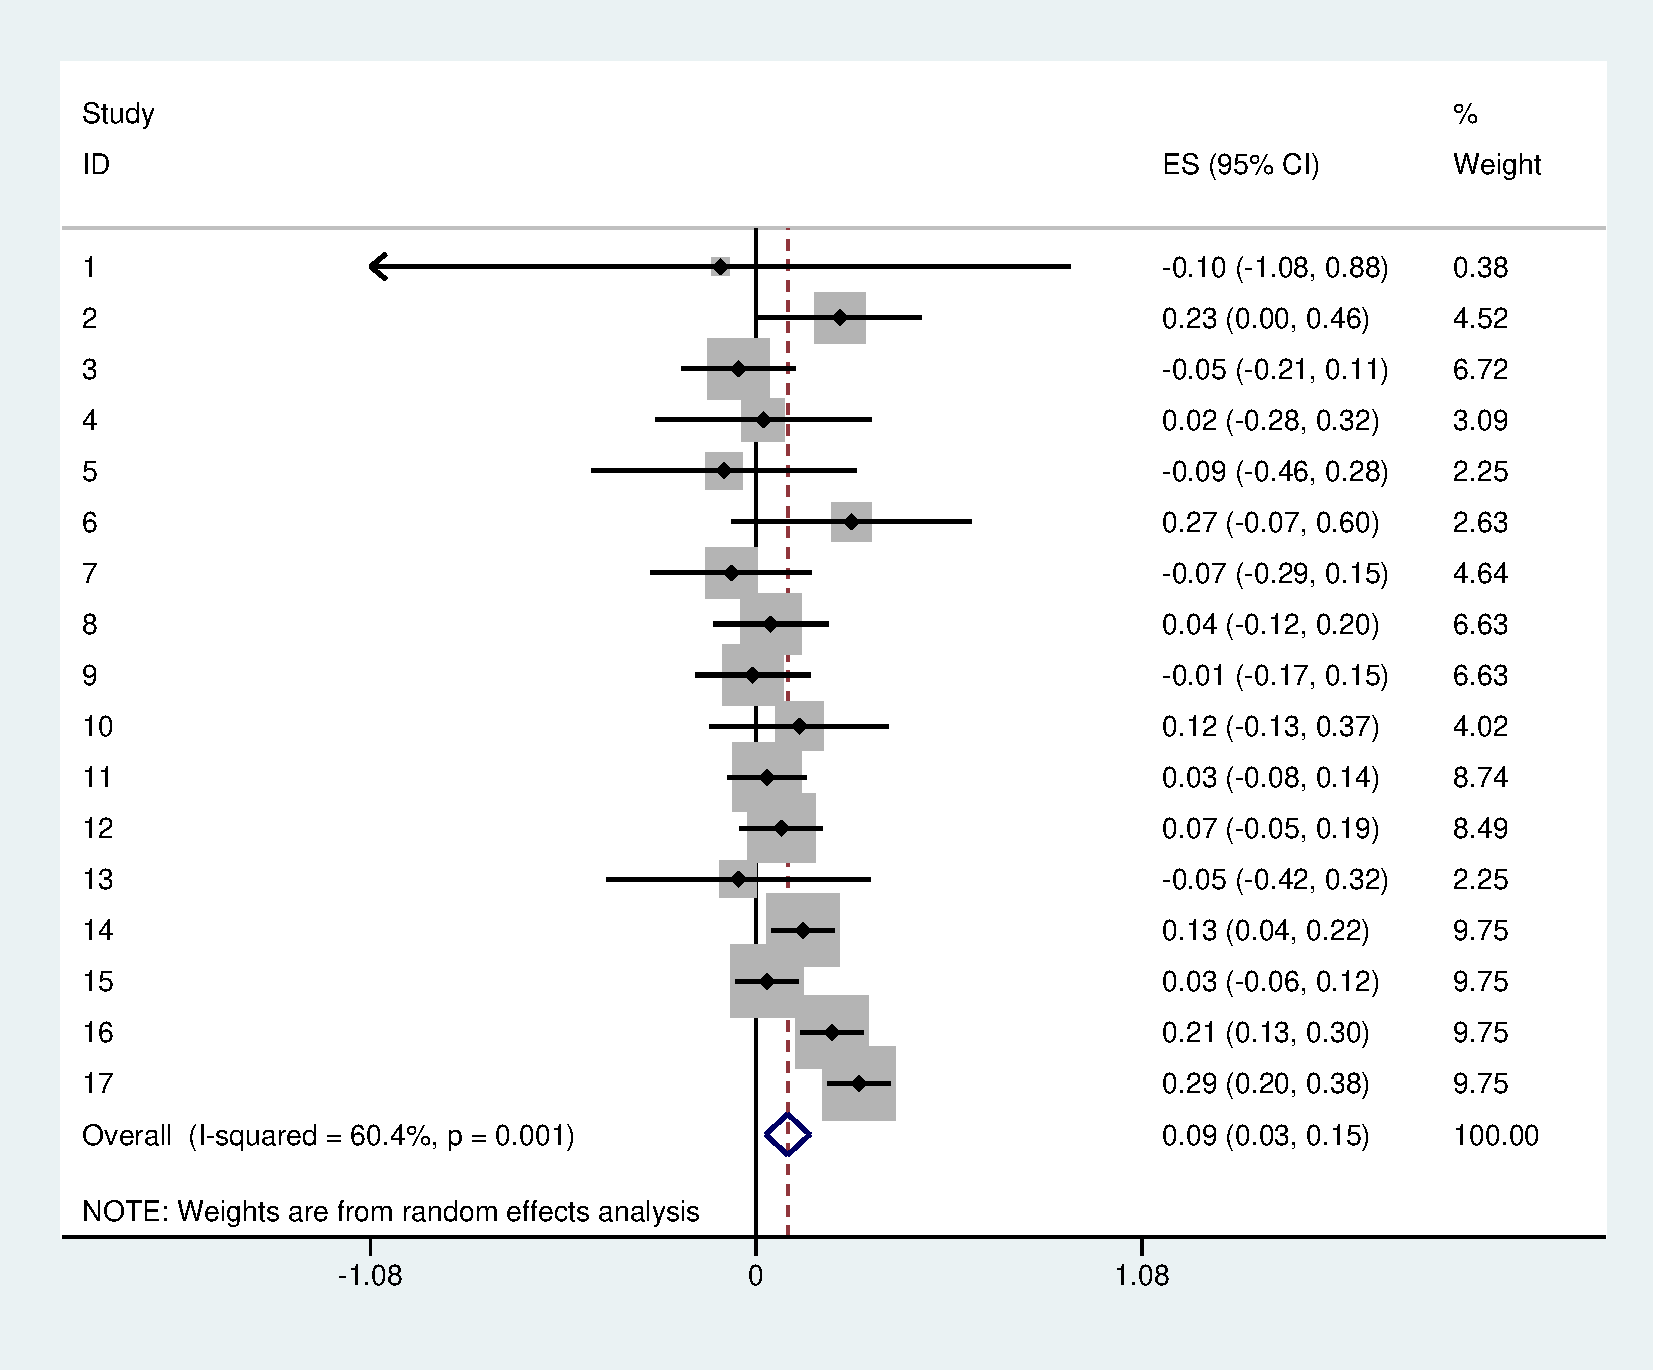
\includegraphics[width=0.8\textwidth]{f_stata_forestplot}
\end{center}

\pagebreak

\section{Übung 2-2}

Nun wird die Durchführung einer sogenannten
Meta-Regression erläutert. Wie bereits im Foliensatz eingeführt, werde ich dafür
einen Datensatz verwenden, in dem die Wirksamkeit des BCG-Impfstoffs zur
Tuberkulosebekämpfung untersucht wird.

In R stellt das Paket \code{metafor} Funktionen (\code{rma()}) zur Meta-Regression bereit. In
Stata ist dafür der Befehl \code{metareg} zuständig (ggf. mit \code{ssc install
  metareg} installieren).


\subsection{Meta-Regression}

\paragraph{Aufgabe 2-2-1} Zunächst muss das Paket \code{metafor} und der
Datensatz geladen werden.\footnote{Der Datensatz ist im Paket \code{metafor}
  enthalten. Die Schritte zum Laden der Daten und der Effektstärkenberechnung
  werden hier aber übersprungen. Weitere Details finden Sie, wenn Sie sich die
  Hilfe für \code{?rma} anschauen.} Die hier verwendete Effektstärke ist das
relative Risiko (genauer: $ln(RR)$), \code{yi}, und deren Varianz
(\code{vi}). Die unabhängige Variable \code{ablat} enthält den Breitengrad als
Maß für den Abstand zum Äquator.

\begin{rbsp}
\begin{knitrout}
\definecolor{shadecolor}{rgb}{1, 1, 1}\color{fgcolor}\begin{kframe}
\begin{verbatim}
library(metafor)
\end{verbatim}


{\ttfamily\noindent\itshape\textcolor{messagecolor}{R>  Loading required package: Formula}}

{\ttfamily\noindent\itshape\textcolor{messagecolor}{R>  Loading 'metafor' package (version 1.6-0). For an overview \\R>  and introduction to the package please type: help(metafor).}}

{\ttfamily\noindent\itshape\textcolor{messagecolor}{R>  \\R>  Attaching package: 'metafor'}}

{\ttfamily\noindent\itshape\textcolor{messagecolor}{R>  The following object(s) are masked from 'package:meta':\\R>  \\R>      forest, funnel, labbe, radial, trimfill}}\begin{verbatim}

dfReg <- read.csv(file = "../../data/dBCG.csv", sep = ";")

## Teile der Tabellenangaben mit -c(1,2,3,9) ausblenden
dfReg[, -c(1,2,3,9)]
R>     tpos  tneg cpos  cneg ablat       yi       vi
R>  1     4   119   11   128    44 -0.88931 0.325585
R>  2     6   300   29   274    55 -1.58539 0.194581
R>  3     3   228   11   209    42 -1.34807 0.415368
R>  4    62 13536  248 12619    52 -1.44155 0.020010
R>  5    33  5036   47  5761    13 -0.21755 0.051210
R>  6   180  1361  372  1079    44 -0.78612 0.006906
R>  7     8  2537   10   619    19 -1.62090 0.223017
R>  8   505 87886  499 87892    13  0.01195 0.003962
R>  9    29  7470   45  7232    27 -0.46942 0.056434
R>  10   17  1699   65  1600    42 -1.37134 0.073025
R>  11  186 50448  141 27197    18 -0.33936 0.012412
R>  12    5  2493    3  2338    33  0.44591 0.532506
R>  13   27 16886   29 17825    33 -0.01731 0.071405
\end{verbatim}
\end{kframe}
\end{knitrout}

\end{rbsp}

Nun können wir mit einem Fixed-effects-Modell beginnen. Wie oben bereits
erwähnt, so heißt die hier verwendete R Funktion \code{rma}. Mit dem Argument
\code{mods = $\sim$ablat} werden die Prädiktoren eingebunden (weitere
Prädiktoren werden mit \code{+} angehängt, also \code{mods =
  $\sim$v1+v2+v3+\ldots}). Schließlich wird mit \code{method} beschrieben,
nach welchem Verfahren die Koeffizienten berechnet werden sollen. Hier steht
\code{"FE"} für das Fixed-effects-Modell.

Zusätzlich wird an diesem Beispiel noch die Verwendung des Befehls
\code{summary} illustriert. Zunächst wird das Ergebnis der Regression im Objekt
\code{bcg.fem} gespeichert und dann mit dem \code{summary}-Befehl
ausgegeben. Wenn Sie einfach die \code{rma}-Funktion aufrufen, dann werden keine
Modellgütestatistiken (Deviance, AIC, BIC) ausgegeben.

Wiederum werden eine Menge Zahlen ausgegeben und die folgenden Fragen sollen
Ihnen helfen, sich zu orientieren:
\begin{itemize}
\item Wo finden Sie die Regressionskoeffizienten des Modells? Sind diese auf dem
  1\%-Niveau statistisch signifikant?
\item Ist das FE Modell angemessen? Wenn nein, warum nicht?
\end{itemize}

\begin{rbsp}
\begin{knitrout}
\definecolor{shadecolor}{rgb}{1, 1, 1}\color{fgcolor}\begin{kframe}
\begin{verbatim}
bcg.fem <- rma(yi = yi, vi = vi, mods=~ablat, method = "FE", data = dfReg)
summary(bcg.fem)
R>  
R>  Fixed-Effects with Moderators Model (k = 13)
R>  
R>    logLik  Deviance       AIC       BIC  
R>   -9.4736   18.9472   22.9472   24.0771  
R>  
R>  Test for Residual Heterogeneity: 
R>  QE(df = 11) = 30.7331, p-val = 0.0012
R>  
R>  Test of Moderators (coefficient(s) 2): 
R>  QM(df = 1) = 121.4999, p-val < .0001
R>  
R>  Model Results:
R>  
R>           estimate      se      zval    pval    ci.lb    ci.ub     
R>  intrcpt    0.3436  0.0810    4.2390  <.0001   0.1847   0.5024  ***
R>  ablat     -0.0292  0.0027  -11.0227  <.0001  -0.0344  -0.0240  ***
R>  
R>  ---
R>  Signif. codes:  0 '***' 0.001 '**' 0.01 '*' 0.05 '.' 0.1 ' ' 1
\end{verbatim}
\end{kframe}
\end{knitrout}

\end{rbsp}

Nach dem Fixed-effects-Modell schätzen wir nun ein Mixed-effects-Modell. Dazu
verwenden wir den \code{DL}-Schätzer (DerSimonian-Laird). Nachfolgend einige
Fragen zu den Ergebnissen der Modellschätzung:
\begin{itemize}
\item Vergleichen Sie die Regressionskoeffizienten zwischen den beiden
  Modellen. Sehen Sie Unterschiede? Vergleichen Sie auch die Standardfehler
  (Spalte \code{se}). Sind die Standardfehler größer oder kleiner geworden?
\item Welche zusätzliche Statistik findet sich nun in der R-Ausgabe?
\item Schließlich die entscheidende Frage: Welches der beiden Modelle würden Sie
  publizieren?
\end{itemize}

\begin{rbsp}
\begin{knitrout}
\definecolor{shadecolor}{rgb}{1, 1, 1}\color{fgcolor}\begin{kframe}
\begin{verbatim}
summary(rma(yi = yi, vi = vi, mods=~ablat, method = "DL", data = dfReg))
R>  
R>  Mixed-Effects Model (k = 13; tau^2 estimator: DL)
R>  
R>    logLik  Deviance       AIC       BIC  
R>   -7.8338   15.6677   21.6677   23.3625  
R>  
R>  tau^2 (estimate of residual amount of heterogeneity): 0.0633
R>  tau (sqrt of the estimate of residual heterogeneity): 0.2516
R>  
R>  Test for Residual Heterogeneity: 
R>  QE(df = 11) = 30.7331, p-val = 0.0012
R>  
R>  Test of Moderators (coefficient(s) 2): 
R>  QM(df = 1) = 18.8452, p-val < .0001
R>  
R>  Model Results:
R>  
R>           estimate      se     zval    pval    ci.lb    ci.ub     
R>  intrcpt    0.2595  0.2323   1.1172  0.2639  -0.1958   0.7149     
R>  ablat     -0.0292  0.0067  -4.3411  <.0001  -0.0424  -0.0160  ***
R>  
R>  ---
R>  Signif. codes:  0 '***' 0.001 '**' 0.01 '*' 0.05 '.' 0.1 ' ' 1
\end{verbatim}
\end{kframe}
\end{knitrout}

\end{rbsp}

Zum Schluß noch die Befehle und die Ergebnisse der Meta-Regression in Stata. In
Stata existiert hierfür die Funktion \code{metareg}, die ggf. noch installiert
werden muss. In Stata gibt es (mind.) zwei Besonderheiten:
\begin{itemize}
\item Ein FE Model wird in Stata mit der Funktion \code{vwls} geschätzt.
\item Stata gibt ein $R^2$ aus.
\end{itemize}


\begin{statabsp}
  \lstinputlisting{../stata/assign-2-2-1.do}
\end{statabsp}


\begin{statabsp}
\begin{tiny}
  \lstinputlisting{../../tab/assign-2-2-1.txt}
\end{tiny}
\end{statabsp}





\subsection{Publication Bias}

Im letzten Übungsteil befassen wir uns mit diagnostischen Verfahren zur
Identifikation eines möglichen Publication Bias.

\paragraph{Aufgabe 2-2-2}  Erstellen Sie mit der Funktion \code{funnel} einen Funnelplot. Als
  Argument übergeben Sie dabei ein \code{meta}-Objekt. Was denken Sie? Liegt ein
  Publication Bias vor? Im Anhang ihres Artikels schreiben Aloe/Becker (2009) dazu:

  \begin{quote}
    \enquote{The funnel plot in Figure 2 shows the 17 data points included in the correlation analysis.
      The EEO-study correlations are the four data points on the top of the graph, with large sample
      sizes in comparison to the other studies.  While this plot was not strongly funnel shaped because
      of the EEO data points, the rest of the values followed a reasonably funnel shaped pattern,
      indicating no publication bias.}
  \end{quote}

  Und, sehen Sie das auch so?

\pagebreak  
  
\begin{rbsp}
\begin{knitrout}
\definecolor{shadecolor}{rgb}{1, 1, 1}\color{fgcolor}\begin{kframe}
\begin{verbatim}
tmp <- metacor(cor = r, n = N, data = dfVerb)
funnel(tmp)
\end{verbatim}
\end{kframe}
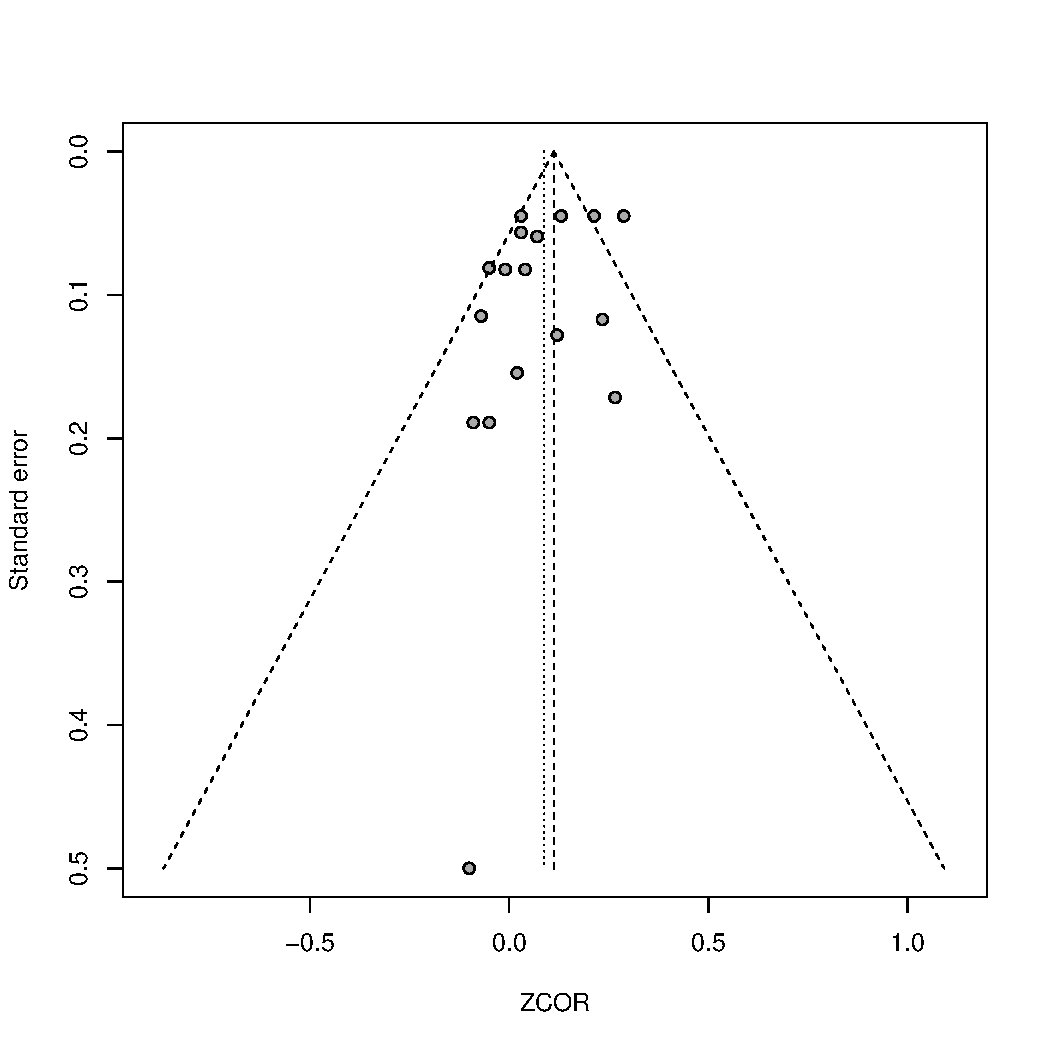
\includegraphics[width=\maxwidth]{fig/assign-2-2-2_1} 

\end{knitrout}

\end{rbsp}


Funnelplots lassen sich natürlich auch mit Stata erstellen. Verwenden Sie hierzu den Befehl \code{metafunnel}.

\begin{statabsp}
  \lstinputlisting{../stata/assign-2-2-2.do}
\end{statabsp}

\begin{center}
  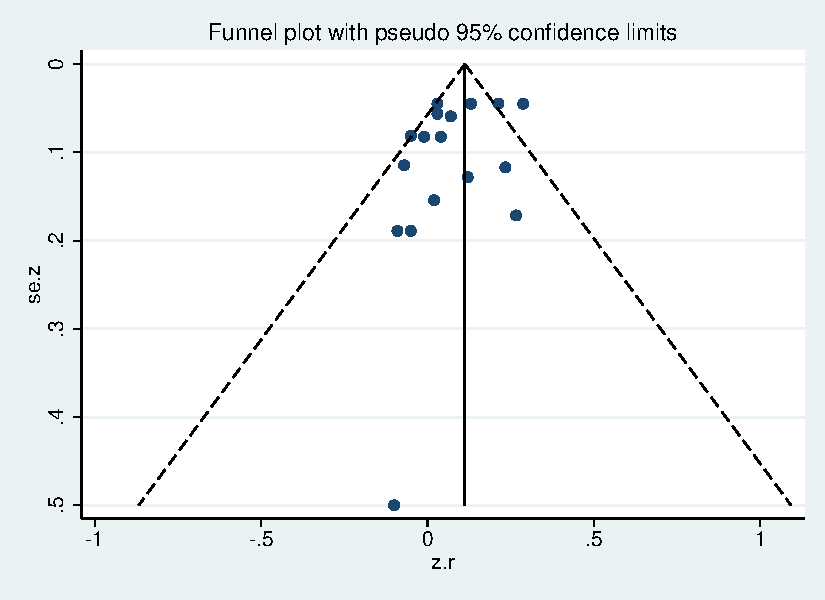
\includegraphics[width=0.8\textwidth]{f_stata_funnelplot}
\end{center}

Funnelplots haben u.a. den Nachteil, dass ihre Interpretation sehr subjektiv
ausfallen kann. Es gibt daher verschiedene statistische Verfahren, mit denen
sich dieser Prozess \enquote{objektivieren} lässt.

Ein gängiger Test ist der Egger-Test, der auf einer einfachen linearen Regression
basiert. Es gibt keinen deutlichen Hinweis auf einen möglichen Publication Bias,
wenn die Regressionsgerade durch den Ursprung läuft, also der Intercept nicht
von Null verschieden ist.

In R gibt es für diese Tests die Funktion \code{metabias} (wiederum Teil des
\code{meta} Paketes). Hier sind verschiedene Tests implementiert und mit dem
Argument \code{ method.bias = "linreg"} wählen wir den Egger-Test.

\pagebreak

Nachfolgend finden Sie die Ergebnisse der Analysen. Was denken Sie, gibt es
Anzeichen für einen Publikation Bias? Unter dem ersten R Beispiel finden Sie
ebenfalls die Befunde einer einfachen linearen Regression. Vergleichen Sie die
Ergebnisse und versuchen Sie die verschiedenen Werte zuzuordnen.

\begin{rbsp}
\begin{knitrout}
\definecolor{shadecolor}{rgb}{1, 1, 1}\color{fgcolor}\begin{kframe}
\begin{verbatim}
## Eggers Regressions-Test durchfuehren
metabias(tmp, method.bias = "linreg")
R>  
R>  	Linear regression test of funnel plot asymmetry
R>  
R>  data:  tmp 
R>  t = -1.429, df = 15, p-value = 0.1736
R>  alternative hypothesis: asymmetry in funnel plot 
R>  sample estimates:
R>     bias se.bias   slope 
R>  -1.1124  0.7786  0.1815
\end{verbatim}
\end{kframe}
\end{knitrout}

\end{rbsp}

\begin{rbsp}
\begin{knitrout}
\definecolor{shadecolor}{rgb}{1, 1, 1}\color{fgcolor}\begin{kframe}
\begin{verbatim}
## Eggers Regressions-Test mit den R-Standard-Funktionen durchfuehren
dfVerb$snd <- dfVerb$z.r/dfVerb$se.z
dfVerb$prec <- 1/dfVerb$se.z

summary(lm(snd ~ prec, data = dfVerb))
R>  
R>  Call:
R>  lm(formula = snd ~ prec, data = dfVerb)
R>  
R>  Residuals:
R>     Min     1Q Median     3Q    Max 
R>  -2.265 -1.081 -0.113  0.637  3.479 
R>  
R>  Coefficients:
R>              Estimate Std. Error t value Pr(>|t|)   
R>  (Intercept)  -1.1124     0.7786   -1.43    0.174   
R>  prec          0.1815     0.0552    3.29    0.005 **
R>  ---
R>  Signif. codes:  0 '***' 0.001 '**' 0.01 '*' 0.05 '.' 0.1 ' ' 1 
R>  
R>  Residual standard error: 1.54 on 15 degrees of freedom
R>  Multiple R-squared: 0.419,	Adjusted R-squared: 0.38 
R>  F-statistic: 10.8 on 1 and 15 DF,  p-value: 0.00498
\end{verbatim}
\end{kframe}
\end{knitrout}

\end{rbsp}

Auch in Stata ist der Egger-Test implementiert. Er wird mit der Funktion \code{metabias} durchgeführt.

\begin{statabsp}
  \begin{tiny}
    \lstinputlisting{../../tab/assign-2-2-2.txt}
  \end{tiny}

\end{statabsp}



\end{document}
